% Название разделов -- все прописные
\section{ПОСТАНОВКА ЗАДАЧИ}

\subsection{Потребность во внедрении электронных интерактивных таблиц дифференциальной диагностики}

Дифференциальная диагностика – это процесс, при котором врач проводит различие между двумя или более заболеваниями, которые могут вызвать наблюдаемые у человека симптомы.

Зачастую не существует лабораторных методов, которые могли бы окончательно поставить причину симптомов заболевания. Это происходит потому, что многие состояния имеют одинаковые или сходные симптомы, а некоторые проявляются по-разному. Чтобы поставить диагноз, врач может использовать метод, называемый дифференциальной диагностикой.

Дифференциальная диагностика включает в себя составление списка возможных состояний, которые могут быть причиной симптомов. Врач будет основываться на информации, которую он получает от:

\begin{itemize}
    \item истории болезни человека;
    \item результатов физического обследования;
    \item диагностического тестирования.
\end{itemize}

Именно значения, полученные одним или несколькими из данных способов, лежат в основе таблиц дифференциальной диагностики. Сопоставляя значения, таблицы могут помочь определить, болен ли человек конкретным заболеванием или нет; они определяют его степень, выраженность, стадию, могут рассчитать объём поражения организма. Также таблицы могут подсказать нормы показателей для разных случаев или возрастов пациентов.

Таблицы представляют собой компактное представление набора симптомов и соответствующего им заболевания. Это очень удобный вид представления информации, так как он помогает вычленить основные моменты и быстрее определить диагноз. Врачам не надо долго искать нужную информацию в учебниках, книгах, или статьях. В связи с чем очень многие врачи (а также студенты или обычные люди) часто пользуются ими для определения чего-либо. Пример таблицы дифференциальной диагностики приведён на рисунке~\ref{fig:tab1}.

\begin{figure}
  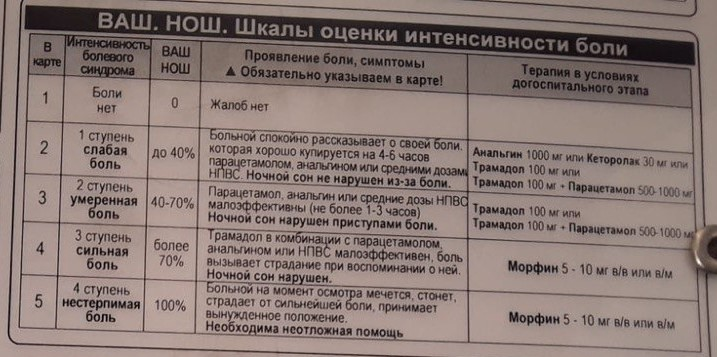
\includegraphics[scale=0.6]{src/ВАШ. НОШ. Шкалы оценки интенсивности боли.jpg}
  \caption{Пример таблицы дифференциальной диагностики}
  \label{fig:tab1}
\end{figure}

Но на данный момент врачи скорой помощи вынуждены носить с собой огромные папки с различными справочными материалами, которые им могут понадобиться в работе, в их числе и таблицы дифференциальной диагностики. В целом данных таблиц существует несколько сотен -- в самых разных отраслях медицины. Физически переносить такой объём материала, очевидно, очень трудно, поэтому врачи скорой помощи носят с собой только самые основные и часто используемые. В остальном им приходится полагаться на свою память. Но даже при таком объёме поиск нужного материала среди них занимает довольно продолжительное время, а время в работе врачей скорой помощи может играть решающую роль. 

Также в целом у всех врачей значительную часть времени отнимает заполнение медицинской карты пациента.

В связи с этим остро стоит потребность цифровизации таблиц дифференциальной диагностики.

Во-первых, это снизило бы физическую нагрузку на врачей, так как у них отпала бы необходимость в переноске объёмных бумажных материалов. Во-вторых, это снизило бы и психологическую нагрузку -- ведь у врачей скорой помощи очень напряжённая работа, и к этому ещё прибавляется беспокойство о том, правильно ли они запомнили показатели той или иной болезни, не забыли ли они чего-либо. С введением цифровых таблиц дифференциальной диагностики  часть этой нагрузки уйдёт. В-третьих, они также позволят снизить процент неправильной постановки диагноза, так как врач сможет найти нужную информацию в данных таблицах. Кроме того в приложении может быть доступ ко многом сотням таблиц, что расширит возможности врачей. И, наконец, это ускорит работу врачей в целом - как и при поиске нужного материала, так и при заполнении медицинской карты пациента, так как результат можно автоматически занести в карту.

\subsection{Анализ существующих подходов к решению проблемы}

Существуют различные представления таблиц дифференциальной диагностики. Первый - это бумажный вариант, который, как показано выше, имеет множество недостатков.

Существуют различные сайты в интернете, где приведены некоторые таблицы дифференциальной диагностики. Пример --  сайт \url{https://medcollege-old.bsu.edu.ru/uchebniki/tabldif.htm}, показанный на рисунке~\ref{fig:tab2}\cite{medcollege}.

\begin{figure}
  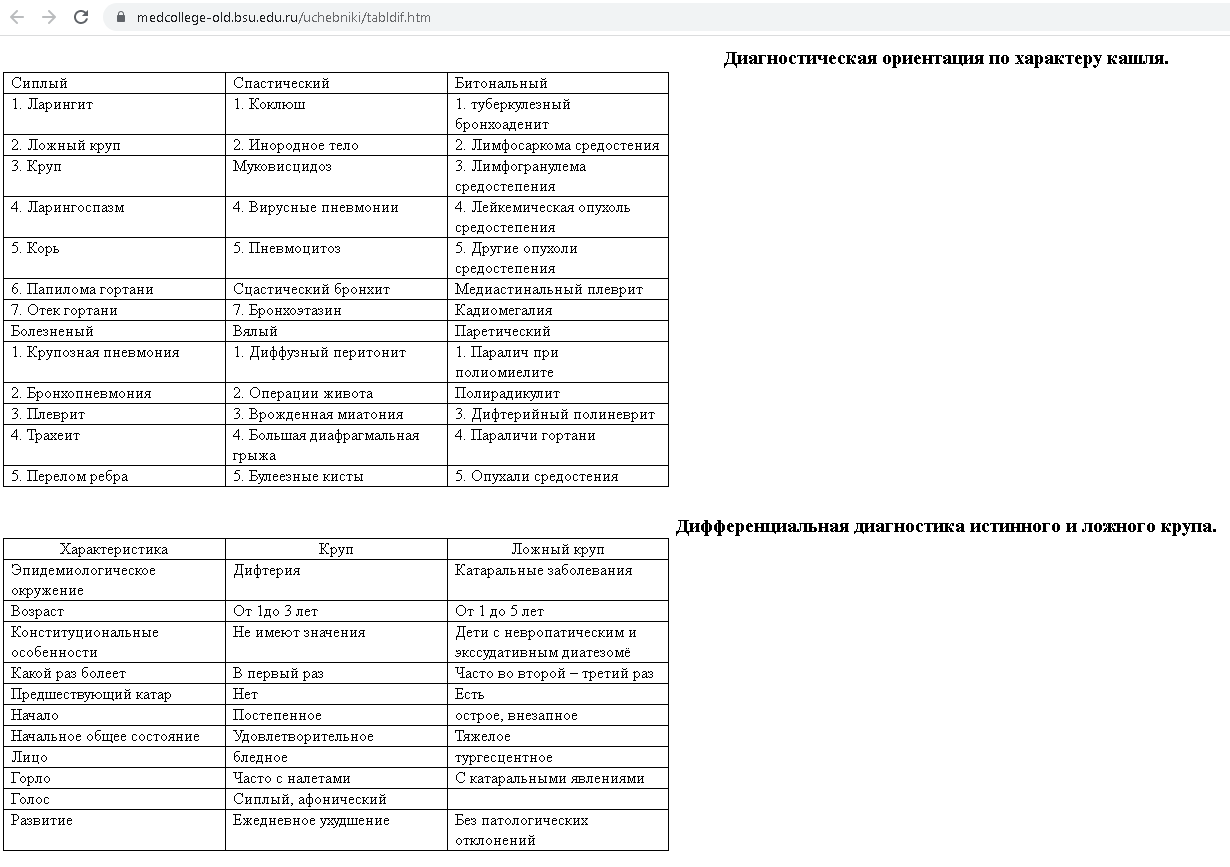
\includegraphics[scale=0.5]{src/extab1.png}
  \caption{Пример сайта с некоторыми таблицами дифференциальной диагностики}
  \label{fig:tab2}
\end{figure}

Но у него есть существенный недостаток, как впрочем, и у остальных подобных сайтов в интернете: в них представлена лишь часть таблиц дифференциальной диагностики, набранных или случайным образом, или в соответствии с тематикой сайта, например "Желудочные заболевания у детей". То есть, нет единого сайта с таблицами дифференциальной диагностики, который бы объединял разные таблицы по разным направлениям -- при использовании сети интернет приходится по одиночке искать нужную таблицу, что также отнимает время. И не всегда таблицу можно найти -- она может быть вообще не представлена в электронном виде, или же существовать лишь в виде нескольких абзацев текста.

Существует также чат-бот помощник в Telegram под названием "PARAMEDIC (шпаргалки)" \cite{paramedic}, который предназначен специально для помощи работникам скорой медицинской помощи. Его вид приведён на рисунке~\ref{fig:bot}(а).  Он выдаёт справочные материалы на самые различные темы во многих отраслях медицины. В том числе в нём есть примеры заполненных медицинских карт, а также множество схем и таблиц дифференциальной диагностики. Его преимущество перед сайтами из интернета заключается в обширности разнообразного материала, систематизированного по категориям. Минус же данного бота в том, что в нём нет поиска по названию --  пользователю приходится переходить несколько раз по множеству папок, ища нужное. Кроме того, его существенный недостаток заключается в том, что данные в нём представлены в совершенно различных форматах -- таблицы и схемы могут быть в виде картинок, файлов с расширением .pdf, в виде ссылки на Яндекс-диск, где хранится множество файлов или же ссылки на другой сайт со статьей по данной теме; пример представлен на рисуннке~\ref{fig:bot}(б). То есть нет единого формата хранения, а пользователь может переходить по совершенно разным ссылкам на другие ресурсы. 

\begin{figure}
  \begin{subfigure}[t]{0.1\linewidth}
    \centering
    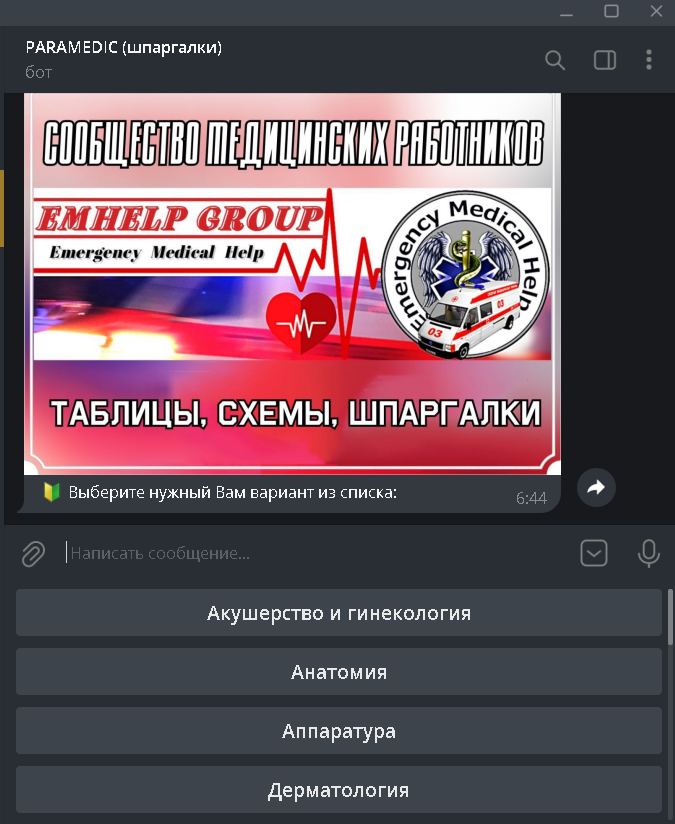
\includegraphics[scale=0.4]{src/exbot1.png}
    \caption{}
  \end{subfigure}
  \hfill
  \begin{subfigure}[t]{0.5\linewidth}
    \centering
    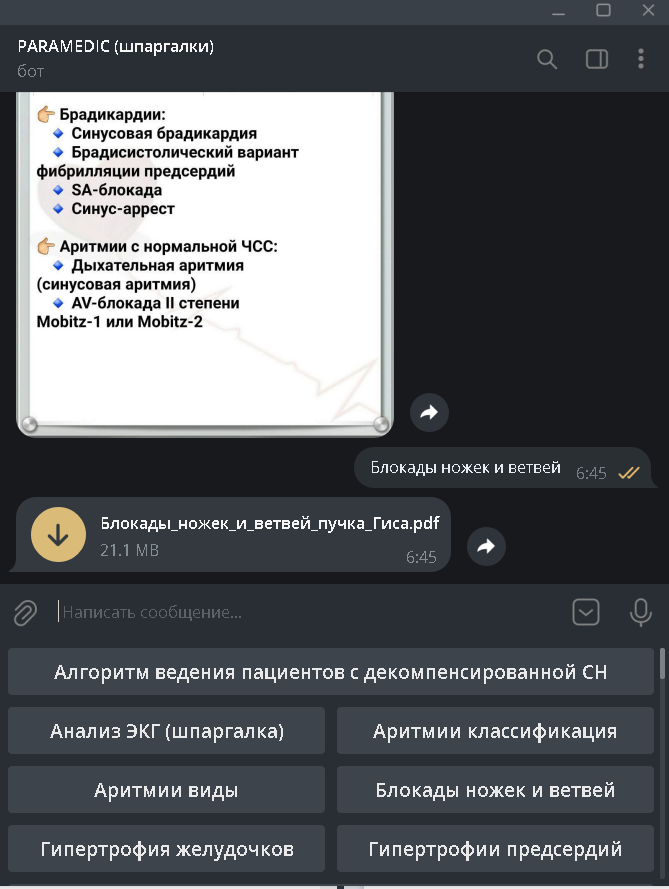
\includegraphics[scale=0.4]{src/exbot2.png}
    \caption{}
  \end{subfigure}
  \caption{Чат-бот "PARAMEDIC (шпаргалки)"}
  \label{fig:bot}
\end{figure}

Также существуют специальные программы, предназначенные для дифференциальной диагностики пациентов.

Одна из таких программ - DiagnosisPro \cite{DiagnosisPro}, представлена на рисунке~\ref{fig:diagpro}. Она была разработана специально для повышения качества медицинской помощи и предотвращения диагностических ошибок.

\begin{figure}
  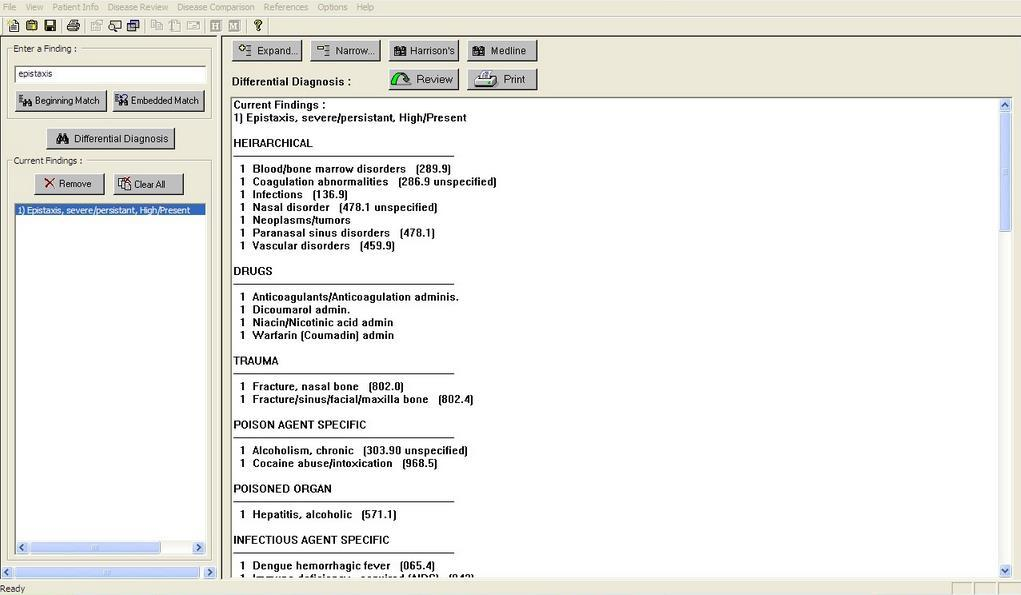
\includegraphics[scale=0.5]{src/diag_pro6.jpg}
  \caption{Программа DiagnosisPro 6.0}
  \label{fig:diagpro}
\end{figure}

Эта программа была очень распространена в США и могла выдавать около 15 000 проявлений заболеваний, таких как симптомы, лабораторные исследования, ЭКГ, рентгеновские снимки, снимки компьютерной томографии, МРТ, УЗИ, патологии, результаты микробиологии и многое другое. 

Как можно понять, она, в том числе, частично реализовывала функцию таблиц дифференциальной диагностики -- выдавала список симптомов болезней. Почему только частично -- потому, что основная цель этой программы немного отличалась от целей таблиц дифференциальной диагностики. Программа позволяла составить список возможных заболеваний и потом постепенно исключить из него неподходящие варианты. Тогда как задача таблиц дифференциальной диагностики -- быстрое определение степени уже выявленного заболевания. Можно сказать, что программа DiagnosisPro решала более общую комплексную задачу дифференциальной диагностики. 

Но у этой программы также есть свои недостатки. Первый, и самый основной, это то, что в 2016 году программа перестала поддерживаться и теперь приобрести её у компании-разработчика невозможно. Вторым недостатком было то, что хотя программа и была бесплатной и свободно распространяемой в медицинской сфере, она поддерживала только английский, испанский, французский, арабский и китайский языки. То есть при работе этой программы в России врачи, не владеющие на достаточном уровне английским языком, не смогли бы пользоваться ею. И даже у врачей, владеющих английским языком, возникли бы проблемы при переводе результатов или симптомов из программы на русский язык для внесения в медицинскую карту пациента. Не говоря уже о том, что это существенно замедлило бы работу врачей.

Существует также ещё одна подобная программа -- VisualDx \cite{visualdx}, сайт которой представлен на рисунке~\ref{fig:vdx}. Она также предназначена для решения общей задачи дифференциальной диагностики: врачи могут составлять индивидуальный план пациента, где, отметив его симптомы и основные сведения о человеке, могут просмотреть возможные диагнозы, предложенные программой. Также в VisualDx делает особый упор на визуализацию -- их библиотека содержит более чем 40 000 фотографий различных заболеваний на коже людей разных национальностей, а также врач может просмотреть различные симптомы или болезни в виде рисунка-анимации.

\begin{figure}
  
\includegraphics[scale=0.3]{src/VisDx.png}
  \caption{Сайт программы VisualDx}
  \label{fig:vdx}
\end{figure}

Но у VisualDx также есть свои минусы. Первый -- она, как и  DiagnosisPro не поддерживает русский язык (только английский, французский, немецкий, китайский, европейский испанский и латиноамериканский испанский языки). Второй -- она платная. Плата вносится ежемесячно или ежегодно, в зависимости от числа компьютеров и пользователей.

И она также, как и DiagnosisPro не реализует электронные таблицы дифференциальной диагностики -- она просто выводит список заболеваний, объясняющих симптомы и различную информацию про эти заболевания. То есть, опять же, решает более глобальную и большую проблему дифференциальной диагностики заболеваний. И таблицы дифференциальной диагностики (или их подобие) присутствуют там лишь в виде текста статьи. Пример такой статьи о распознавании синяков и ушибов на теле детей приведён на рисунке~\ref{fig:vdx_ex_ac}. В обычных случаях это помогает врачу поставить более точный диагноз, глубже разобраться в проблеме, тщательнее изучить тему. Но врачам скорой помощи приходится принимать решения быстро, чаще всего у них нет времени читать статьи и находить среди них нужную информацию. Им надо быстро определить степень заболевания, площадь ожогов, вероятность сердечного приступа у человека и т.п. Именно в таких случаях полезнее информация, содержащая только основные моменты и представленная в виде интерактивных таблиц.
 
\begin{figure}
  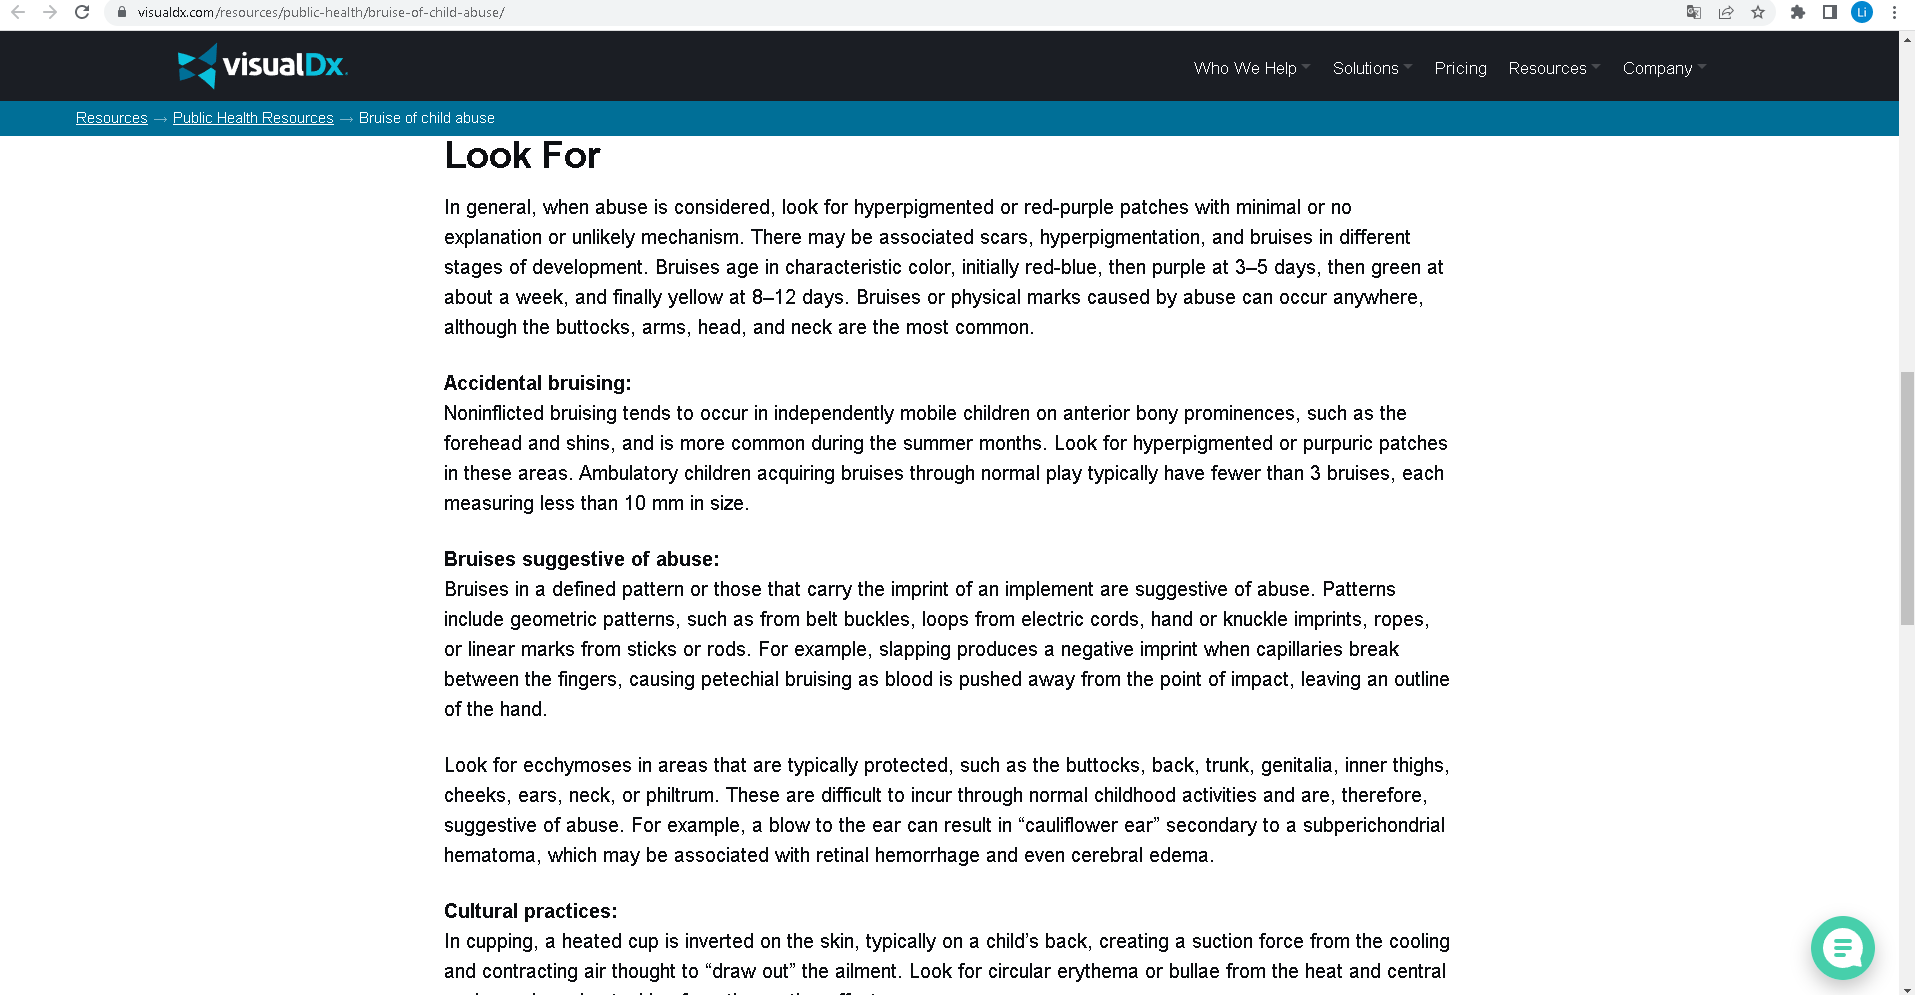
\includegraphics[scale=0.3]{src/vdx_ex_article.png}
  \caption{Статья VisualDx о распознавании синяков и ушибов на теле детей}
  \label{fig:vdx_ex_ac}
\end{figure}

\subsection{Обоснование цели и задач, техническое задание на разработку}

В связи со всем вышесказанным моей целью стало разработать интерактивные таблицы дифференциальной диагностики, учтя все минусы и плюсы существующих решений. 

В России существует веб-приложение \url{onmp.ru} \cite{onmp}. Его изображение представлено на рисунке~\ref{fig:onmp0}. Оно создано специально для заполнения медицинских карт врачами скорой помощи и в нём учтены все спецификации формы медицинской карты вызова. В нём можно заполнять медицинские карты, сохранять их, откладывать в черновики, шаблоны или архив. Оно было разработано сотрудниками и студентами Московского Авиационного Института. Таким образом, можно внедрить таблицы дифференциальной диагностики в это приложение, сделать это отдельной его функцией. 

\begin{figure}
  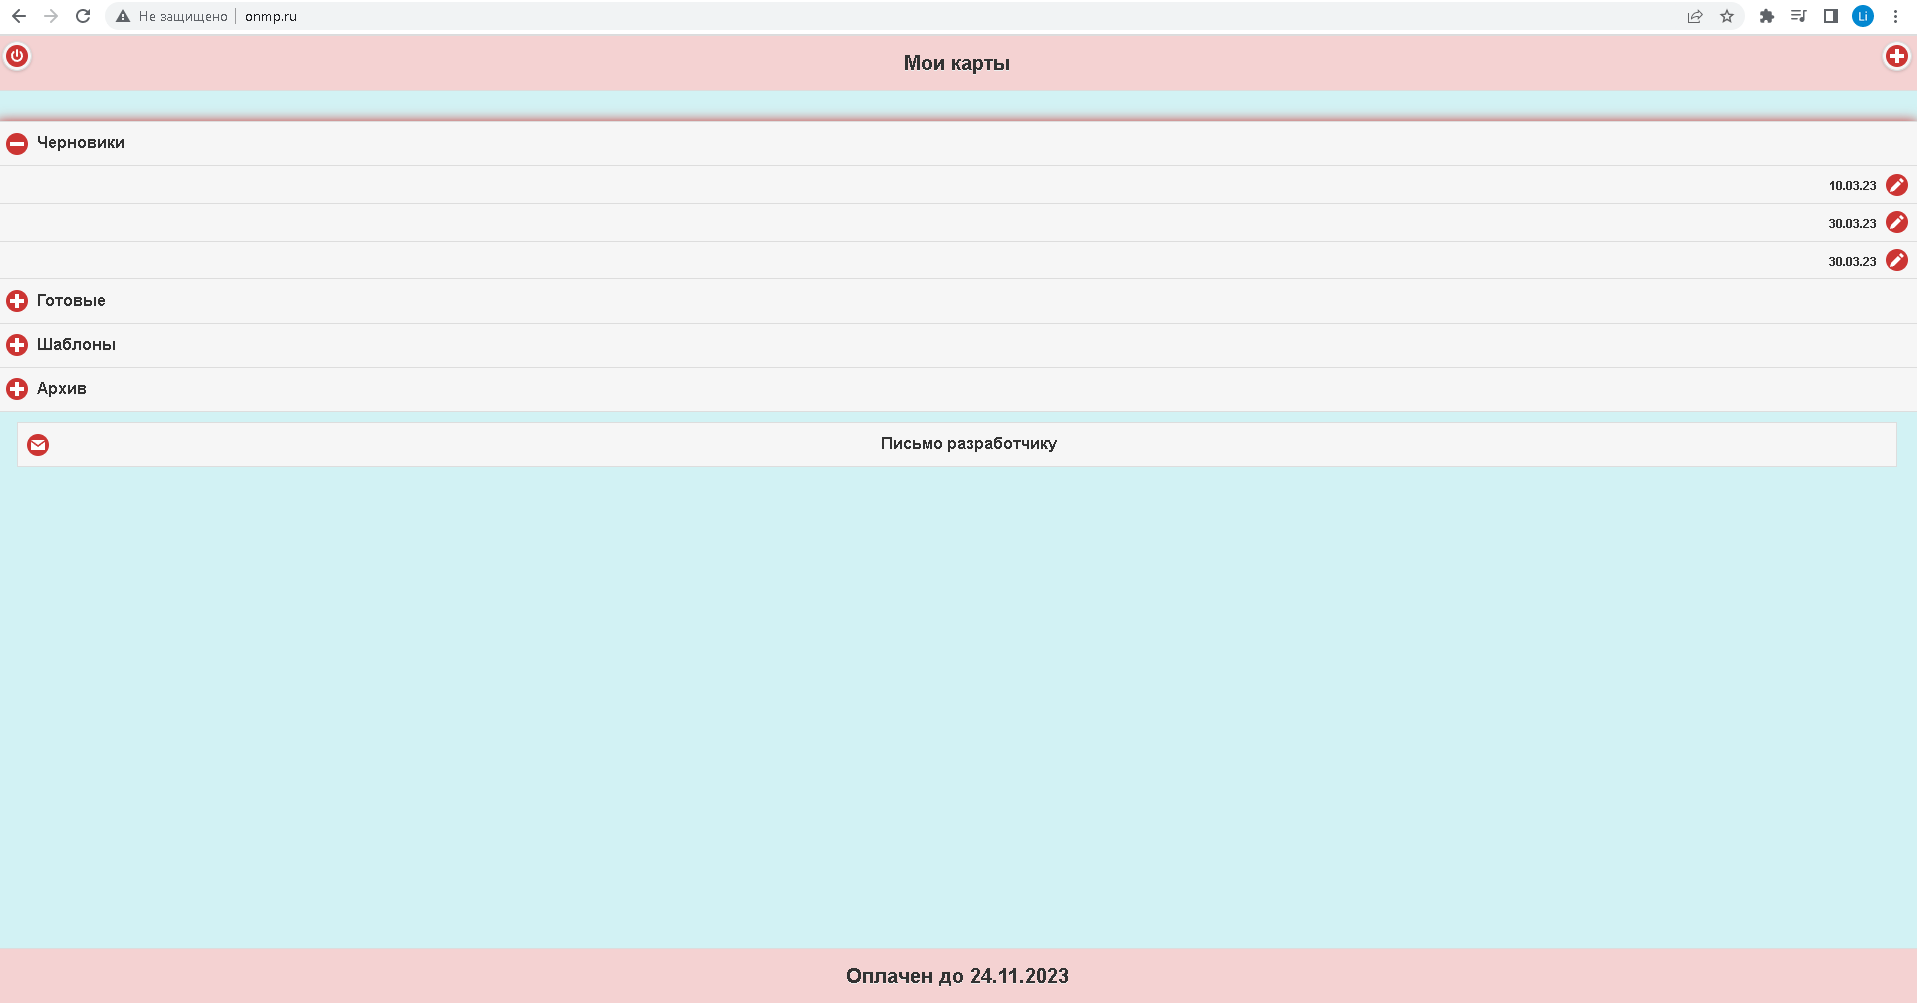
\includegraphics[scale=0.3]{src/onmp0.png}
  \caption{Сайт onmp.ru}
  \label{fig:onmp0}
\end{figure}

Таким образом мы решим две проблемы предыдущих решений. Во-первых, приложение ОНМП поддерживает русский язык, так как в первую очередь ориентированно именно на Российских врачей, а также в нём настроена форма заполнение такой формы медицинской карты вызова, которую предусматривает законодательство Российской Федерации. Во-вторых, это приложение бесплатно, в отличии от инестранных аналогов.

Теперь разберём более детально, что надо учесть при внедрении таблиц дифференциальной диагностики.

Чтобы обеспечить врачам доступ к всесторонней информации, надо внедрить большое количество таблиц дифференциальной диагностики. Следовательно, для их хранения надо использовать базу данных и разработать метод их хранения в ней.  Этим мы решим проблемы тех сайтов, на которых представлено лишь малое количество таблиц дифференциальной диагностики, и которые не справятся с иными случаями.

Чтобы врачи могли быстро найти нужную таблицу, надо реализовать быстрый поиск по названиям этих таблиц. Этим мы решим проблему долгого поиска среди бумажных листов, в интернете и в телеграм-боте.

Чтобы было удобно работать с таблицами, надо реализовать функцию интерактивной работы с ними -- например, дать возможность пользователю выбирать симптомы в строках или баллы в столбцах.

Чтобы снизить психологическую нагрузку на врачей, также надо реализовать автоматический расчёт результата. Это также снизит вероятность ошибки врачом.

И, наконец, так как приложение \url{onmp.ru} создано специально для заполнения медицинских карт пациентов, то надо реализовать функцию автоматического внесения результата в медицинскую карту пациента (а именно в поле Status localis). Это также позволит врачам немного быстрее заполнять медицинские карты.

Итак, цель работы: внедрение медицинских таблиц дифференциальной диагностики в веб-приложение \url{onmp.ru}.

Она состоит из следующих задач:

\begin{enumerate}
  \item Внедрить 20 таблиц дифференциальной диагностики, для хранения использовать базу данных.
  \item Реализовать быстрый поиск по таблицам.
  \item Реализовать интерактивную работу с таблицами.
  \item Реализовать автоматический подсчёт результата.
  \item Создать функцию автоматической записи результата в медицинскую карту пациента.
\end{enumerate}